\section{Conventions and an audited positivity obstruction}
All algebras and Hilbert spaces in this note are over $\C$. Put $q=u^2>0$
and $\kappa=u-u^{-1}$. The normalized finite Hecke algebra $H_q(S_3)$ has
basis $T_e=1,T_s=S,T_t=T,T_{st}=ST,T_{ts}=TS,T_{sts}=STS$, with
\begin{equation}\label{eq:p2-relations}
 S^*=S,\quad T^*=T,\quad S^2=1+\kappa S,\quad
 T^2=1+\kappa T,\quad STS=TST.
\end{equation}
Thus $T_w^*=T_{w^{-1}}$ and $\tau(T_w)=\delta_{w,e}$ is a faithful tracial
state: $\tau(x^*x)=\sum_w|x_w|^2$ for $x=\sum_wx_wT_w$.
The faithful left regular representation on the six-dimensional Hilbert
space with orthonormal basis $T_w$ realizes the C*-algebra. No completion
ambiguity occurs in finite dimension. The unnormalized generators
$H_s=uT_s$ satisfy $(H_s-q)(H_s+1)=0$; diagonal rescaling does not change
the multipliers considered here.

Write $\ell(w)$ for Coxeter length and $\Phi_r(T_w)=r^{\ell(w)}T_w$,
$0\leq r\leq1$. We use the Heisenberg convention: a QMS consists of unital
CP maps preserving the specified trace, and its evolution generator is
$L$ in $\exp(tL)$. In finite dimension continuity is norm continuity.
Diagonal real rates are $L^2(\tau)$-symmetric and trace preserving, but
these properties alone do not imply positivity.

\begin{theorem}[Audited obstruction]\label{thm:p2-obstruction}
For $q>0$, $q\ne1$, the map $\Phi_{e^{-t}}$ is not positive whenever
$0<t<\frac12|\log q|$. At $q=4$, $e^{-t}=3/4$, a positive central
projection has an image with eigenvalue exactly $-1/210$.
The same interval obstructs the restricted length formula in any reduced
Coxeter Hecke C*- or von Neumann algebra with a standard $A_2$ parabolic
whose two generators have common parameter $q\ne1$; in particular it
applies to equal-parameter affine $\widetilde A_2$.
\end{theorem}
\begin{proof}
Suppose first $q>1$. Define
\[
 P(q)=(1+q)(1+q+q^2),\qquad
 Z=1+u(S+T)+u^2(ST+TS)+u^3STS,\qquad p_+=Z/P(q).
\]
For each pair $w,sw$ with $\ell(sw)=\ell(w)+1$, the multiplication rule
gives $S(T_w+uT_{sw})=u(T_w+uT_{sw})$. Multiplying by $u^{\ell(w)}$
and summing gives $SZ=uZ$, and similarly $TZ=uZ$. Hence
$T_wZ=u^{\ell(w)}Z$, $Z^2=P(q)Z$, and $Z^*=Z$. Thus $p_+^2=p_+^*=p_+$
and $\tau(p_+)=1/P(q)>0$: the witness is a positive projection by direct
algebraic verification. Right multiplication proves centrality as well.

Define a two-dimensional representation $\pi_0$ by
\begin{equation}\label{eq:p2-matrices}
 B_s=\begin{pmatrix}u&0\\0&-u^{-1}\end{pmatrix},\qquad
 B_t=\frac1{q+1}\begin{pmatrix}-u^{-1}&\sqrt{q^2+q+1}\\
                  \sqrt{q^2+q+1}&uq\end{pmatrix}.
\end{equation}
Both matrices are selfadjoint; direct multiplication verifies all three
relations in~\eqref{eq:p2-relations}. Set $B_w=\pi_0(T_w)$ and
$J=B_s+B_t-\kappa I_2$. The same multiplication gives
$J^*=J$, $J^2=I_2$, and $\Tr J=0$. Expansion in $r$ yields the useful
factorization
\begin{equation}\label{eq:p2-witness-factor}
 \pi_0(\Phi_r(p_+))=
 \frac{(1-r)(1+qr)}{P(q)}(I_2+urJ).
\end{equation}
For example this identity can be verified coefficient by coefficient:
insert $B_s,B_t,B_sB_t+B_tB_s,B_sB_tB_s$ on the left. Since the eigenvalues
of $J$ are $1,-1$, the two eigenvalues are exactly
\[
 \lambda_\pm(q,r)=\frac{(1-r)(1+qr)(1\pm ur)}{P(q)}.
\]
The minus branch is negative for $u^{-1}<r<1$, as claimed.
At $u=2,r=3/4$, the image and its negative eigenvector are
\[
 X=\begin{pmatrix}8/525&\sqrt{21}/350\\\sqrt{21}/350&2/525\end{pmatrix},
 \qquad v=\begin{pmatrix}-\sqrt{21}/7\\1\end{pmatrix},
 \qquad Xv=-v/210.
\]
Its other eigenvalue is $1/42$. These are exact identities.

For $0<q<1$, use the trace-preserving *-isomorphism
\[
 \iota_q:H_q(S_3)\longrightarrow H_{1/q}(S_3),\qquad
 \iota_q(T_w^{(q)})=(-1)^{\ell(w)}T_w^{(1/q)}.
\]
Generator negation changes the quadratic coefficient from $\kappa$ to
$-\kappa$; both sides of every braid have the same length, so the signs
agree. The map respects the involution and coefficient trace, and its
inverse is the same rule with the parameters exchanged. It intertwines
$\Phi_r$ on every basis vector. The different positive witness is
\[
 p_-^{(q)}=\frac{\sum_w(-u^{-1})^{\ell(w)}T_w^{(q)}}{P(1/q)},
 \qquad \iota_q(p_-^{(q)})=p_+^{(1/q)}.
\]
The preceding projection proof transports exactly (or repeats with
the sign eigenvalue $-u^{-1}$). In the representation
$\pi_0^{(1/q)}\circ\iota_q$ the negative eigenvalue is
$\lambda_-(1/q,r)$ for $\sqrt q<r<1$. The factor $1-\sqrt q\,r$
from the first witness is not negative in this case and is not used.

For the affine or broader stated consequence, the span of $T_w$ for
$w\in W_J\simeq S_3$ is a genuine unital *-subalgebra. The left regular
action of its generators on $\ell^2(W_J)\subset\ell^2(W)$ is the faithful
finite regular representation; the subspace is reducing. The algebraic
embedding into the ambient regular representation is therefore faithful,
and a faithful *-homomorphism from this finite C*-algebra is isometric.
Standard-parabolic length agrees with ambient length, so the diagonal
multiplier restricts to the same $\Phi_r$. Positivity would restrict to
positivity on this C*-subalgebra, a contradiction. The representation
$\pi_0$ need not extend to the ambient algebra. The broader assertion
requires positive admissible parameters and exactly such an equal-parameter
standard $A_2$ parabolic; no claim about every non-right-angled system follows.
\end{proof}

At $t=0$ the map is the identity for every $q$. At $q=1$, Coxeter length
is conditionally negative definite, so the usual group Fourier semigroup
is UCP at every time. At $t=|\log q|/2$ the displayed negative branch is
zero, and this witness supplies no failure. Nor does it establish positivity
or CP at the threshold or later times. The proved open interval is not a
classification of isolated positive or CP multipliers. At $r=0$ the map
is $\tau(\cdot)1$ and is UCP. No endpoint inference is needed to rule out
the proposed semigroup.

\subsection{E003: independent reconstruction and scope audit}
\paragraph{Goal} Turn the historical certificate into a self-contained,
independently reproducible theorem without changing the checkpoint.
\paragraph{Hypothesis} The projection calculation survives an independent
reconstruction, with parameter inversion essential below $q=1$.
\paragraph{Method} A reviewer was given only the algebra relations,
conventions and claimed interval, and reconstructed the witness and
representation before reading earlier scripts or proofs. The coordinator
reran both historical exact scripts and reconciled the scope.
\paragraph{Implementation} The new independent artifact is
\texttt{scripts/verify\_obstruction\_review.py}; its review is
\texttt{scripts/results/review\_phase2.txt}. The mathematical source is
shared by this note and \texttt{report.tex}, avoiding divergent proofs.
\paragraph{Results}
{\setlength{\tabcolsep}{8pt}\renewcommand{\arraystretch}{1.2}
\begin{tabular}{lll}\toprule
Check & Result & Evidence\\\midrule
Historical symbolic and regular scripts & Pass & Exact arithmetic\\
Fresh projection/representation derivation & Pass & Equation~\eqref{eq:p2-witness-factor}\\
$q<1$ witness and basis signs & Pass & Explicit $\iota_q(p_-)=p_+$\\
Threshold and finite-parabolic scope & Delimited & No claim past witness interval\\
Bibliographic discrepancy & Corrected annotation & BCW latest version is v3\\\bottomrule
\end{tabular}}
\paragraph{Analysis} No mathematical disagreement was found in the
historical obstruction. The old review's final version sentence called BCW
v2 current, despite the main report correctly citing v3; the new source
audit corrects that record. BCW Assumption 8.1 (published p.~543) assumes
the UCP property, while Problem 9.1 (p.~546) asks about the word-length
case within a broader approximation-property problem~\cite{BorstCaspersWasilewski2024}.
Our obstruction addresses that particular assumed multiplier family, not
the broader Haagerup or completely bounded approximation properties.
The generic warning about transporting group CND functions is already
present in Borst's 2021 thesis, Section 8.2, p.~39~\cite{BorstMSc2021}.
Borst's 2025 dissertation still records the generality question in
Assumption 4.7.1, p.~86, and Problem 4.8.1, p.~90~\cite{BorstPhD2025}.
The latest inspected BCW is arXiv v3, 10 September 2024; its repairs to
Lemmas 3.5--3.6 do not change the question being addressed.
Klisse--Perovi\'c remains a 2025 preprint (v1, listed to appear), whose
Section 5.3 distinguishes ambient Schur maps from maps on the deformed
algebra~\cite{KlissePerovic2025}. None of these inspected passages gives
the exact obstruction or the cone below. The audit also checked focused
forward/backward neighbors through 30 September 2026; it is not a complete
MathSciNet/zbMATH or unpublished-priority audit.
An explicit exact certificate and a self-contained proof have been established
here. Whether the theorem itself is new remains unconfirmed by the bounded
literature search; failure to find it is not proof of originality.
\paragraph{Next steps} Classify the finite diagonal generator cone and
separate genuinely global affine conclusions from local tests.
\begin{verification}
\textbf{What:} Relations, projection, factorization, rational eigenvalue,
and parameter-inversion witness.\\
\textbf{Method:} Exact symbolic and faithful regular algebra calculations;
the affine embedding is proved above, not inferred from samples.\\
\textbf{Commands:} \texttt{uv run python scripts/verify\_a2\_explore.py},
\texttt{uv run python scripts/verify\_hecke.py}, and
\texttt{uv run python scripts/verify\_obstruction\_review.py}.\\
\textbf{Outcome:} Exact checks pass; no floating-point tolerance is used.
\end{verification}

\section{The complete finite diagonal generator cone}
\subsection{The C*-algebra and its trace}
In addition to $\pi_0$ in~\eqref{eq:p2-matrices}, let
$\pi_+(T_w)=u^{\ell(w)}$ and $\pi_-(T_w)=(-u^{-1})^{\ell(w)}$.
The map $\Gamma=\pi_+\oplus\pi_-\oplus\pi_0$ identifies the algebra with
\begin{equation}\label{eq:p2-blocks}
 \mathcal A=\C\oplus\C\oplus M_2(\C),\qquad
 \tau(x)=\gamma_+x_++\gamma_-x_-+\gamma_0\Tr_2(x_0),
 \quad
 (\gamma_+,\gamma_-,\gamma_0)=
 \left(\frac1{P(q)},\frac{q^3}{P(q)},\frac q{1+q+q^2}\right).
\end{equation}
Here $\Tr_2$ is unnormalized. For verification, $\Tr B_s=\Tr B_t=\kappa$,
$\Tr B_{st}=\Tr B_{ts}=-1$ and $\Tr B_{sts}=0$. Substitution shows that
the positive weighted trace in~\eqref{eq:p2-blocks} takes value one on
$T_e$ and zero on the other five basis elements. It therefore equals
the faithful coefficient trace. Consequently $\Gamma$ is injective;
both algebras have dimension six, proving the claimed isomorphism.
In particular the weights of the two scalar projections are
$\gamma_+,\gamma_-$, and the total weight of the matrix block is
$2\gamma_0$, not $\gamma_0$.

We allow all four inverse-symmetric rates
\begin{equation}\label{eq:p2-rates}
 a(e)=0,\quad a(s)=x,\quad a(t)=y,\quad
 a(st)=a(ts)=z,\quad a(sts)=v,\qquad x,y,z,v\geq0.
\end{equation}
Set $L(T_w)=-a(w)T_w$. Unitality, trace preservation and $L^2$-symmetry
are automatic; complete positivity of $e^{tL}$ is the remaining issue.

\begin{lemma}[Direct-sum generator criterion]\label{lem:p2-ccp}
Let $\mathcal A=\bigoplus_\alpha M_{d_\alpha}$ and let $L$ be a
Hermiticity-preserving linear map with $L(1)=0$. Define the domain-first
Choi matrices
\[
 C_{\alpha\beta}(L)=\sum_{i,j=1}^{d_\beta}
 E_{ij}\otimes L_{\alpha\beta}(E_{ij}),\quad
 \Omega_\alpha=\sum_{i=1}^{d_\alpha}e_i\otimes e_i,\quad
 Q_\alpha=I-\frac{|\Omega_\alpha\rangle\langle\Omega_\alpha|}{d_\alpha}.
\]
Then $e^{tL}$ is UCP for every $t\geq0$ if and only if
$C_{\alpha\beta}(L)\geq0$ for $\alpha\ne\beta$ and
$Q_\alpha C_{\alpha\alpha}(L)Q_\alpha\geq0$ for every $\alpha$.
\end{lemma}
\begin{proof}
For a map between direct sums, complete positivity is equivalent to CP
of every source-to-target block map. Each such condition is ordinary
Choi positivity. At $t=0$, the off-diagonal Choi blocks of $e^{tL}$ are
zero; the diagonal ones are $|\Omega_\alpha\rangle\langle\Omega_\alpha|$.
Differentiate quadratic forms on their kernels to obtain necessity.

Conversely take a CP map $\Psi$ whose cross blocks equal those of $L$
and whose diagonal Choi matrices are $Q_\alpha C_{\alpha\alpha}(L)Q_\alpha$.
For a Hermitian matrix $C$, $C-QCQ$ has the form
$|\Omega\rangle\langle b|+|b\rangle\langle\Omega|$.
Indeed with $d=\|\Omega\|^2$, take
$b=C\Omega/d-\Omega\langle\Omega,C\Omega\rangle/(2d^2)$.
Reshaping $b$ as a matrix shows that the corresponding linear map is
$X\mapsto BX+XB^*$. Therefore
$L(X)=\Psi(X)+BX+XB^*$ with block diagonal $B$.
The map $e^{t\Psi}$ is CP by its power series; the exponential of the
drift is $X\mapsto e^{tB}Xe^{tB^*}$. The finite-dimensional Trotter
product proves complete positivity of $e^{tL}$.
Finally $L(1)=0$ implies $e^{tL}(1)=1$. This is the direct-sum form of
the standard conditional-Choi criterion; see also Wolf,
Propositions 7.2--7.3, pp.~122--124~\cite{Wolf2012}.
\end{proof}

\begin{theorem}[Full four-rate spectrahedron]\label{thm:p2-cone}
For every $q>0$, the rates~\eqref{eq:p2-rates} generate a trace-preserving
symmetric QMS if and only if the following scalar and three real symmetric
linear matrix inequalities hold:
\begin{align}
 x+y-2z+v&\geq0,\label{eq:p2-scalar}\\
 F_+&=-u(xB_s+yB_t)-u^2z(B_{st}+B_{ts})-u^3vB_{sts}\geq0,\label{eq:p2-fplus}\\
 F_-&=u^{-1}(xB_s+yB_t)-u^{-2}z(B_{st}+B_{ts})+u^{-3}vB_{sts}\geq0,\label{eq:p2-fminus}\\
 K&=-U^*\big[xB_s\otimes B_s+yB_t\otimes B_t
       +z(B_{st}\otimes B_{st}+B_{ts}\otimes B_{ts})
       +vB_{sts}\otimes B_{sts}\big]U\geq0,\label{eq:p2-K}
 \intertext{where the columns of the following matrix are orthonormal:}
 U&=\frac1{\sqrt2}\begin{pmatrix}1&0&0\\0&1&1\\0&1&-1\\-1&0&0\end{pmatrix}.
 \nonumber
\end{align}
The sizes are respectively $1,2,2,3$. This is an explicit spectrahedral
description of the entire requested four-parameter family, without
assuming $x=y$ or omitting transitions between irreducible summands.
\end{theorem}
\begin{proof}
Orthonormality of the Hecke basis gives Fourier inversion
$X=\sum_w\tau(T_w^*X)T_w$. Thus the Choi block, with target $\alpha$
and source $\beta$, is exactly
\begin{equation}\label{eq:p2-fourier-choi}
 C_{\alpha\beta}(L)=-\gamma_\beta\sum_w
 a(w)\overline{\pi_\beta(T_w)}\otimes\pi_\alpha(T_w).
\end{equation}
The conjugation here is entrywise; it is not a transpose. Indeed
$\Tr(B^*E_{ij})=\overline{B_{ij}}$.
Our representations are real. The two scalar cross blocks are positive
weights times $x+y-2z+v$. The scalar-to-matrix and reverse blocks are
positive weights times $F_+$ or $F_-$. The remaining diagonal matrix block
compresses to $\gamma_0K$ on $\Omega_0^\perp$, because $U^*U=I_3$ and
$U^*\Omega_0=0$. Scalar diagonal blocks have zero-dimensional compressions
and impose no further condition. Lemma~\ref{lem:p2-ccp} proves equivalence.
The diagonal real rates preserve $\tau$ and give selfadjoint $L$ on
$L^2(\tau)$; exponentiation preserves these properties.
\end{proof}

\begin{corollary}[Symmetric rates: seven halfspaces]\label{cor:p2-symmetric}
Suppose $x=y=a$, $z=b$, $v=c$, with $a,b,c\geq0$. Define
\[
 k=q+q^{-1}-1,\quad m_+=a(1-q)+bq,\quad
 d_+=\sqrt q\,[a+b(q-1)-cq],
\]
\[
 m_-=a(q-1)+b,\qquad d_-=[aq+b(1-q)-c]/\sqrt q.
\]
The necessary and sufficient inequalities are
\begin{equation}\label{eq:p2-seven}
 2a-2b+c\geq0,\quad a+b-c\geq0,\quad k(b-a)+c\geq0,
 \quad m_+\geq|d_+|,\quad m_-\geq|d_-|.
\end{equation}
The last two absolute-value conditions each comprise two linear halfspaces.
\end{corollary}
\begin{proof}
With $J=B_s+B_t-\kappa I$ as above,
$B_{st}+B_{ts}=-I+\kappa J$ and $B_{sts}=-J$.
Consequently $F_+=m_+I-d_+J$ and $F_-=q^{-1}(m_-I+d_-J)$,
so their eigenvalues are $m_+\pm d_+$ and $q^{-1}(m_-\pm d_-)$.
For completeness the $3\times3$ pencil has the explicit form
\[
 K=\begin{pmatrix}A&B&0\\B&C&0\\0&0&2a-2b+c\end{pmatrix},
\]
\[
 A=\frac{-a(q^4+1)+b(q^4+2q^2+1)+c(q^3+q)}{q(q+1)^2},
 \quad
 B=\frac{\sqrt{q^2+q+1}\,[a(q^2+1)-b(q-1)^2-2cq]}{\sqrt q(q+1)^2},
\]
\[
 C=\frac{2aq+2b(q^2+1)-c(q^2+1)}{(q+1)^2}.
\]
The trace of the upper block is
$a+b-c+k(b-a)+c$, and its determinant is
$(a+b-c)[k(b-a)+c]$, by direct expansion.
Its eigenvalues are therefore $a+b-c$ and $k(b-a)+c$.
Together with the scalar cross condition this proves~\eqref{eq:p2-seven}.
\end{proof}

At $q=4$ the seven inequalities, after positive rescaling, are exactly
\[
 -a+10b-8c\geq0,\quad -5a-2b+8c\geq0,\quad
 2a+5b+c\geq0,\quad 10a-b-c\geq0,
\]
\[
 a+b-c\geq0,\quad -13a+13b+4c\geq0,\quad 2a-2b+c\geq0.
\]
Thus the old provisional list was correct, including sufficiency now
proved. If $a=1,b=2$, its exact range is $2\leq c\leq19/8$.
For $q=1$,~\eqref{eq:p2-seven} reduces to
$b\geq|a-c|$ and $2a-2b+c\geq0$, besides nonnegative rates.
For arbitrary four rates at $q=1$, the theorem agrees with the group
criterion that $(a(g^{-1}h))_{g,h\in S_3}$ be nonpositive on the
zero-sum subspace. That familiar condition alone is insufficient at
$q\ne1$, as the length example shows.

\begin{corollary}[Sharp uniform depolarizing repair]\label{cor:p2-repair}
For $h\geq0$, set $a(w)=\ell(w)+h\,1_{\{w\ne e\}}$. This generates
a QMS on $H_q(S_3)$ exactly when
\begin{equation}\label{eq:p2-repair}
 h\geq h_{\min}(q)=(\sqrt Q-1)(1+Q),\qquad Q=\max(q,q^{-1}).
\end{equation}
In particular $h_{\min}(4)=5$, $h_{\min}(2)=3(\sqrt2-1)$ and
$h_{\min}(1)=0$.
\end{corollary}
\begin{proof}
The trace-depolarizing generator $D(X)=\tau(X)1-X$ has all nonidentity
rates one. In the three pencils it contributes $I_2,I_2,I_3$ and adds
one to the scalar condition. Substituting $(a,b,c)=(1+h,2+h,3+h)$ gives
the seven eigenvalue branches
\[
 h+(1+q)(1\pm\sqrt q),\qquad
 h+(1+q^{-1})(1\pm q^{-1/2}),\qquad
 1+h,\quad h,\quad k+3+h.
\]
The only negative branch at $h=0$ is the minus branch in the first pair
when $q>1$, or in the second pair when $q<1$. The exact threshold is
therefore~\eqref{eq:p2-repair}. At equality every required matrix is PSD,
so the criterion proves the boundary case as well. Below it a cross-block
Choi matrix has a strictly negative eigenvalue, giving necessity without
a numerical optimizer.
\end{proof}

The depolarizing rates $a(w)=h$ for $w\ne e$ are valid for every $h\geq0$:
$e^{t hD}=e^{-th}\id+(1-e^{-th})\tau(\cdot)1$. Length alone corresponds
to $(a,b,c)=(1,2,3)$ and fails whenever $q\ne1$.
A different valid replacement is $(1,2,2)$, obtained from
$L=(E_{\{s\}}-\id)+(E_{\{t\}}-\id)$, where $E_J$ is the
trace-preserving parabolic expectation. This changes only the longest-word
rate. These are different noise prescriptions; the minimum in
Corollary~\ref{cor:p2-repair} refers specifically to adding the same
constant to every nonidentity rate.

\subsection{E004: exact cone and repair}
\paragraph{Goal} Classify the finite generator family and compute an exact
minimum repair, including cross-summand complete positivity.
\paragraph{Hypothesis} Fourier inversion and the direct-sum conditional-Choi
criterion give a tractable spectrahedron; exchange symmetry may linearize it.
\paragraph{Method} Derive the trace weights and block criterion first,
then factor the characteristic polynomials symbolically. All six Hecke
basis elements are retained; the model is the full finite C*-algebra.
\paragraph{Implementation} \texttt{scripts/verify\_generator\_cone.py}
checks trace orthonormality, all nine identity-Choi blocks, the reduced
pencils, the symmetric characteristic polynomials and all repair branches.
It also checks five exact undeformed CND benchmarks, including a failing
case. The reviewer independently reconstructs the criterion and formulas.
\paragraph{Results}
{\setlength{\tabcolsep}{8pt}\renewcommand{\arraystretch}{1.2}
\begin{tabular}{lll}\toprule
Family & Exact answer & Status\\\midrule
All four inverse-symmetric rates & One scalar, two $2\times2$, one $3\times3$ LMI & Proved\\
Exchange-symmetric rates & Seven halfspaces & Proved\\
$q=4$, $(a,b)=(1,2)$ & $c\in[2,19/8]$ & Exact\\
Length plus uniform correction & Equation~\eqref{eq:p2-repair} & Sharp, proved\\
Trace depolarization & Every $h\geq0$ & Established benchmark\\
$q=1$ CND comparison & Five exact matching tests & Verification only\\\bottomrule
\end{tabular}}
\paragraph{Analysis} The previous unverified radial cone is now certified,
and the general four-rate family is covered. One intermediate coordinate
choice used columns with Gram matrix $\operatorname{diag}(2,1,1)$;
that congruence preserves positivity but not ordinary eigenvalues. The
final proof and sharp repair use the orthonormal $U$ above. Thus no
incorrect identity shift or numerical optimum is used. The general CCP
method is standard; the explicit specialized classification is proved
here, with originality unconfirmed.
\paragraph{Next steps} Apply the finite inequalities as necessary local
tests in affine $\widetilde A_2$ and determine the scope of a genuinely
global construction route.
\begin{verification}
\textbf{What:} Full four-rate Choi reduction, seven halfspaces, and sharp
depolarizing threshold.\\
\textbf{Method:} Exact SymPy identities and characteristic polynomials;
finite rational edge checks supplement the symbolic proof.\\
\textbf{Command:} \texttt{uv run python scripts/verify\_generator\_cone.py}.\\
\textbf{Outcome:} Pass. Results and SymPy version are recorded in
\texttt{scripts/results/generator\_cone.json}. No floating-point tolerance
or semidefinite optimization is involved; samples do not prove sufficiency.
\end{verification}
\begin{figure}[ht]
\centering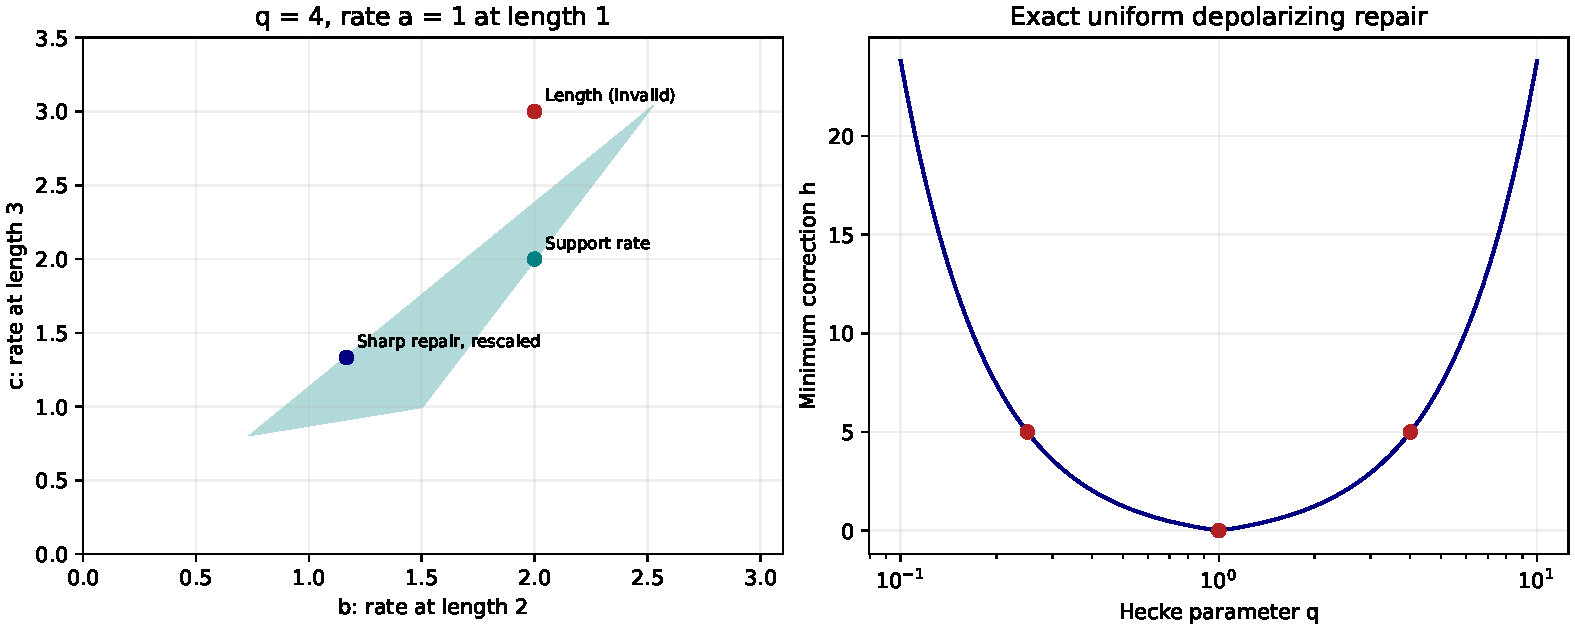
\includegraphics[width=\linewidth]{images/generator_cone.pdf}
\caption{Proved finite-algebra cone and repair formulas. Polygon vertices
are exact rational halfspace intersections; plotting uses floating-point
coordinates only for rendering. The rescaled repaired rates at $q=4$ are
$(a,b,c)=(1,7/6,4/3)$, obtained by dividing $(6,7,8)$ by six.}
\end{figure}
